\section{Knowledge}
\label{sec:knowledge}

A person uploads documents and the assistant answers from them, with each
claim pointing at the passage that states it (Fig.~\ref{fig:knowledge}).

\begin{figure*}[t]
\centering
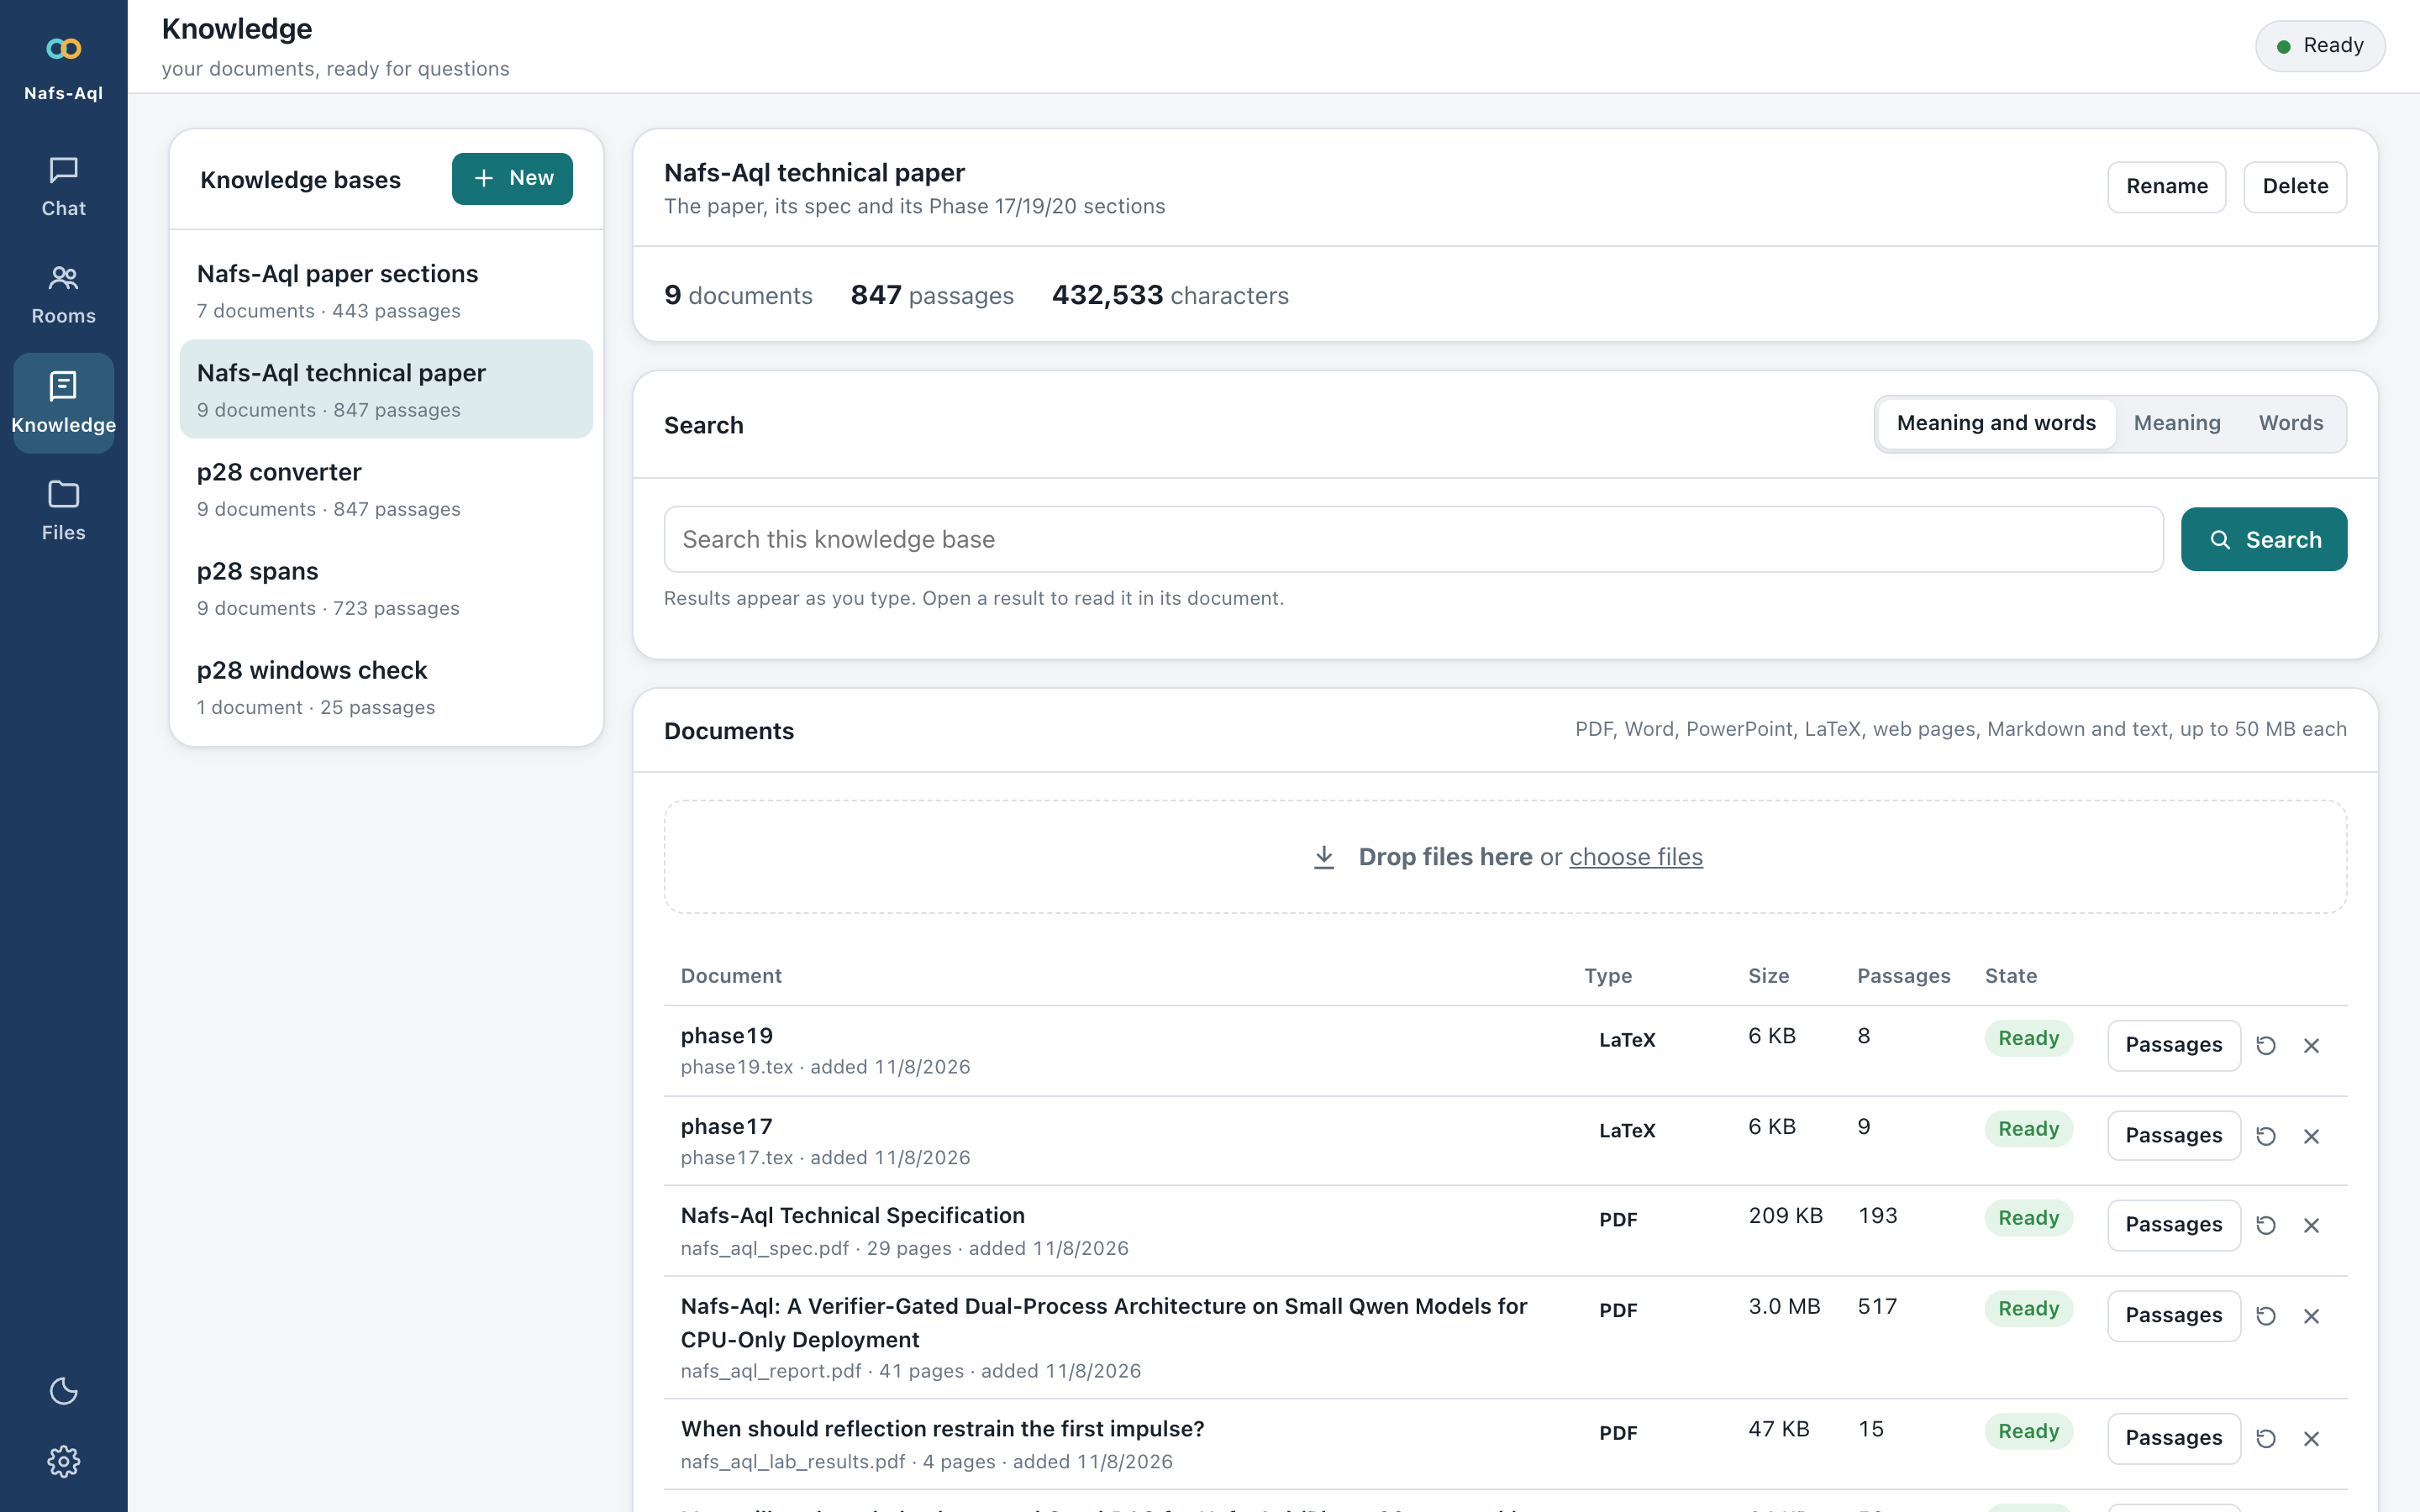
\includegraphics[width=0.48\textwidth]{../shared/screenshots/knowledge.png}\hfill
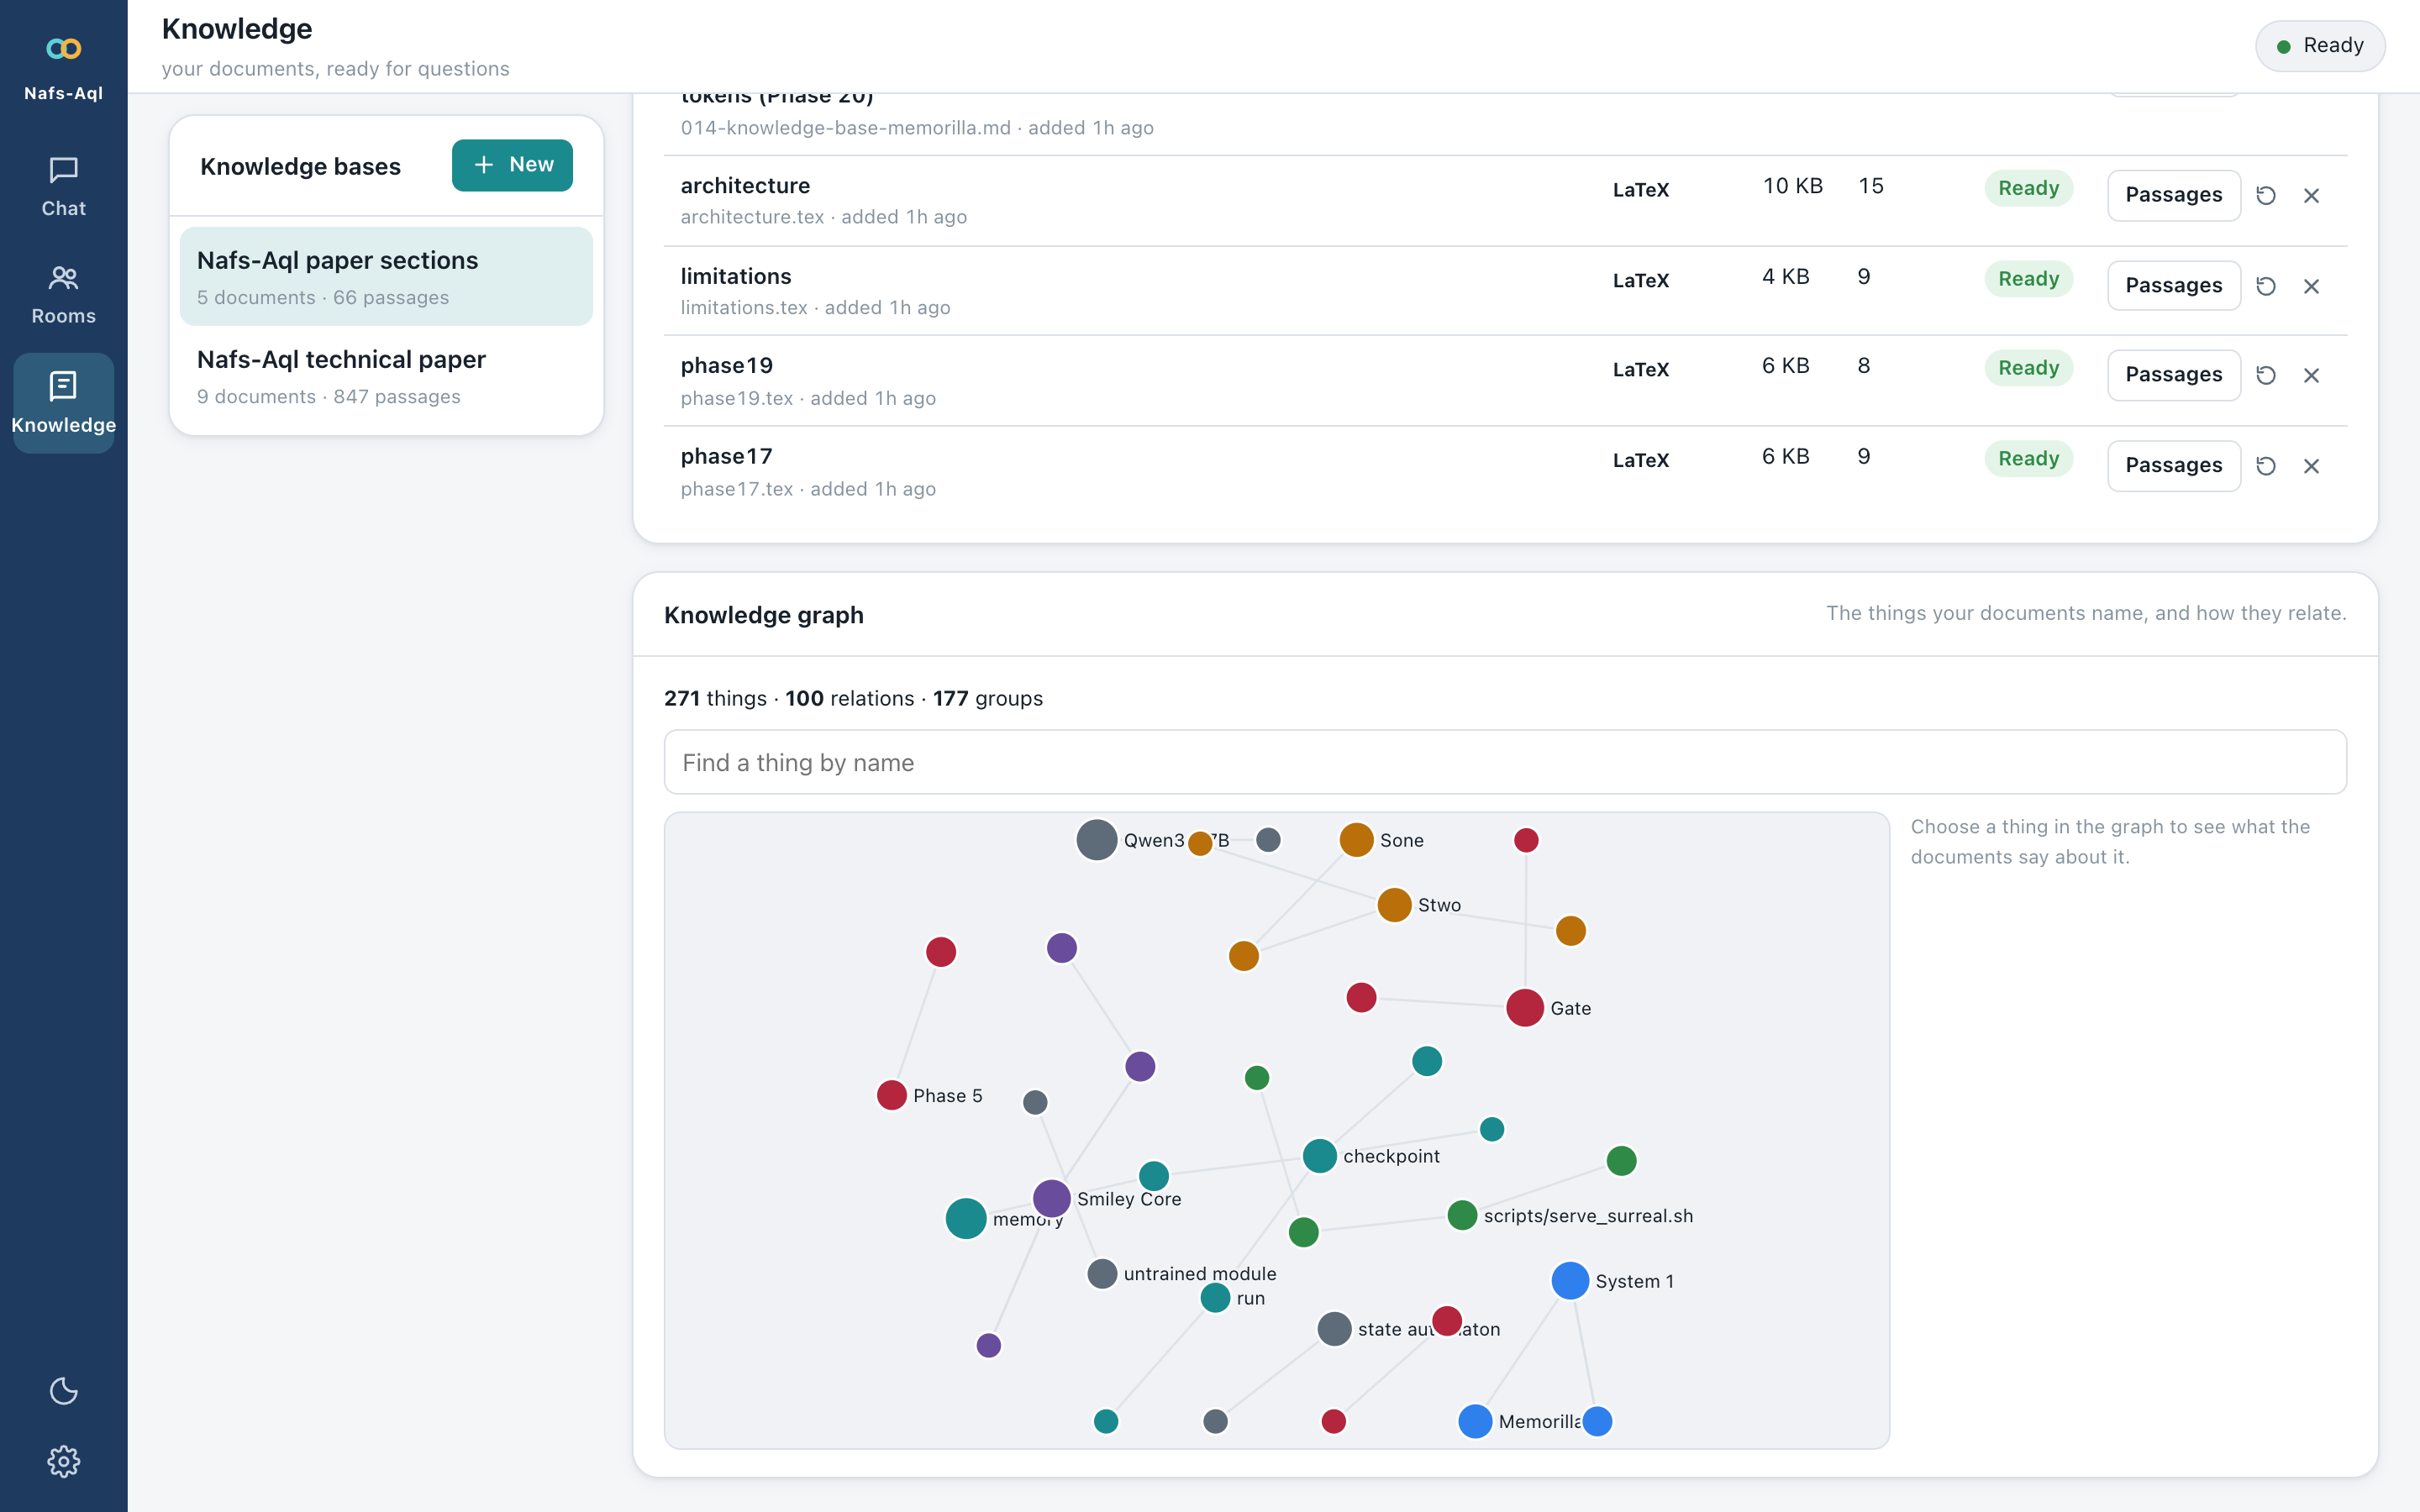
\includegraphics[width=0.48\textwidth]{../shared/screenshots/knowledge_graph.png}
\caption{The Knowledge page with this paper's own sources uploaded (left) and
the graph read from them (right).}
\label{fig:knowledge}
\end{figure*}

\subsection{Reading and storing}
\label{sec:kb:ingest}
Readers written in Rust handle PDF, Word, PowerPoint, \LaTeX, HTML, Markdown
and plain text. A heading-aware chunker cuts passages of 1{,}200 characters
with 150 of overlap, each carrying its heading path and page.

\textbf{Reading a PDF page.} A PDF holds positioned runs of text, not
paragraphs. A layout pass, our Rust rewrite of LiteParse's rules
\cite{liteparse2026} over the reader's runs (box, size, weight, style), turns
them into Markdown in reading order. Columns are found by recursive XY-cut: a
gutter is a valley in the character density of a region's narrow lines, and
the lines that cross it (a title, an abstract, a wide caption) are cut off
first as bands, so the columns are read one after the other. A region whose
rows split into three or more aligned cells is a table and is not cut into
columns; its rows are written as Markdown rows, so a row stays one line.
Running headers and page numbers are removed by position and repetition;
paragraphs are rejoined across line-end hyphens, column breaks and footnotes;
headings come from sizes above the body size, from numbering (``I.'',
``A.'', ``2.5'') in bold, italic or capitals, and from short bold blocks.
Table-of-contents entries are not headings. If the pass fails on a document,
the reader's own converter reads it. On 25 papers (421 pages) parsing and
chunking take 15.5\,ms a page. SurrealDB is the source of
truth for documents, passages, vectors and graphs. Passages are embedded by
Qwen3-Embedding-0.6B, served by the same engine with a pooling head; a
re-read keeps the vector of every passage whose embedded text did not change,
and the embedder keeps the cache rows of the tokens a text shares with the
previous one (every question starts with the same instruction), which leaves
the vectors identical. Ingestion runs on two lanes: parsing, chunking and
storing on a fast lane that makes a document searchable by its words within
seconds, and vectors and the model-built graph on a slow lane, one job at a
time. Uploads are size-capped while streaming, archive budgets do not trust
header sizes, queues, documents per base, passages per file and parser time
are bounded, and deleting a base removes the originals, the passages and the
passages copied into stored replies.

\subsection{An in-process index}
\label{sec:kb:index}
Search does not go to the store. The service holds, per base and per
document, the passages, an inverted index over their words, their vectors and
the terms they name, within a memory limit (512\,MB by default; a base that
does not fit keeps the store's own BM25 and HNSW indexes). A base is
immutable once made and swapped on change, so a search in flight keeps a
consistent view; a change touches one document's part; a generation counter
keeps a load from installing rows read before a change; and every 30\,s, off
the search path, the index's counts are compared with the store's and the
documents that differ are read again.

\textbf{Words.} BM25F over four fields (title, heading path, context line,
body; $k_1=1.2$, $b=0.5$) with lowercase, ASCII folding and Snowball stems,
and one addition: an identifier is a term of its own beside its parts, so
\texttt{vector\_weight} or \texttt{Qwen3-1.7B} is not cut into words that
match everywhere. Function words are left out of a query. The indexed text is
the text a passage is embedded as, including a one-line context
\cite{anthropic2024contextual}. A question word of five letters or more that
the base does not hold is taken for a typing slip and replaced by the nearest
word the base does hold: same first letter, one edit away (two for a word of
eight letters or more, an adjacent swap counting as one), the commonest of the
nearest, at 0.7 of the weight of a word found as typed. Identifiers and
numbers are never corrected.

\textbf{Meaning.} An exact scan of the normalised vectors. Below a few hundred
thousand passages an exact scan is both the fastest and the most accurate
index (100{,}000 vectors of 1{,}024 dimensions in 20.8\,ms here). A base
records the embedding model that wrote its first vector; if another model is
running, the base is searched by its words and says so, until its meaning
index is rebuilt, because vectors of two models are not comparable even at
the same width.

\textbf{Sentence windows.} A passage's vector averages everything the passage
says, so a question about one of its sentences can sit far from it. Each
passage is therefore also cut into windows of about 240 characters (whole
sentences; table rows and list items kept whole), each embedded with the
passage's title and heading path. A passage's meaning score is the mean of
its own similarity and the larger of that and its best window's, an idea taken
from semtools' line-level search \cite{semtools2026} but kept at the level of
the passage, which is what the prompt receives.

\textbf{Fusion.} The two rankings are fused by reciprocal rank
\cite{cormack2009rrf} ($k=60$) with the meaning arm weighted 0.1. A passage
whose lexical score reaches 10.0 is kept whatever its similarity; otherwise a
passage must reach a minimum similarity to be shown to the model, so an
off-topic question retrieves nothing rather than noise.

\subsection{A graph with no model call}
\label{sec:kb:textgraph}
Terms are read from the text by rule: acronyms, identifiers, runs of
capitalised words, and single capitalised words that are also capitalised
away from the start of a sentence. A term named by at least two passages and
at most a fifth of the base is a node, linked to the passages that name it
with a weight that grows with its rarity. For an 847-passage base this gives
1{,}306 terms and 5{,}975 links in under a millisecond, so every base has a
map the moment a file is read. Personalized PageRank over this bipartite
graph (20 rounds of power iteration, seeded by the best passages of the
search and the terms the question names) is available as a third ranking and
serves the graph mode of chat.

\subsection{A graph read by the model}
\label{sec:kb:modelgraph}
On request, the quick model reads each passage once under a JSON Schema and
returns entities, typed relations, a one-line context and the sentence that
states each relation. Entities are merged by name and by the cosine of their
name vectors ($\ge0.92$), relations by their endpoints with a weight, and
Louvain communities are detected. Three rules keep it faithful. Every word of
an entity's name must occur in the passage. A relation is stored only with a
sentence that occurs in its passage verbatim after whitespace normalisation,
which also bounds what a document can put into a prompt through the graph.
The entity types are data stored with the base (an ontology that a person can
edit), and a stray type is mapped onto a declared one. In graph mode,
passages cited by a fact join the candidate pool and the graph's ranking is
fused with the search's as one more arm over the whole pool; a two-hop walk
keeps the best eight relations per reached entity, scored by weight times 0.6
per hop, and shows the chain. Treating the graph as an arm rather than an
override was the decisive change (Section~\ref{sec:eval:knowledge}).
Extraction costs 17 to 28\,s per passage on this machine, so this layer is
opt-in; the rule-built graph is always there.

\subsection{Answering}
\label{sec:kb:chat}
Chat has the modes \texttt{rag} (numbered passages), \texttt{graph},
\texttt{memory}, \texttt{hybrid}, \texttt{auto} and \texttt{off}. Retrieved
text is delimited and labelled as data, never instructions. A sentence packer
fills one character budget with whole units: each sentence is scored by its
own relevance to the question (idf-weighted overlap) plus its passage's rank,
both normalised, and a unit that does not fit is skipped rather than cut.
Every reply names the searches that ran and why any did not, and a numbered
citation opens its passage in context.

\textbf{Follow-up questions.} ``And how fast is it?'' names nothing a search
can find. A question is read together with the previous user turn when it has
fewer than three content words, or when it carries a reference word or an
opening such as ``what about'' and at most six content words; a phrase that
announces a new subject turns the rule off. The rule is a reduction of the
topic-continuity signal of vLLM Semantic Router \cite{semanticrouter2026} to
the one decision needed here, and uses no model.

\textbf{Is the answer in its sources?} An answer written from passages has no
exact verifier, so it carries the lowest assurance level. It is nevertheless
compared with what it was given, sentence by sentence and with no model.
Citation marks, list numbers, questions and sentences that decline (``the
passages do not say'') are set aside. A remaining sentence is \emph{supported}
when at least 60\,\% of its stemmed content words are in one passage or
repeated from the question, and every number it states occurs in the passages
or in the question, with ``1{,}200'' equal to ``1200'' and ``four'' to
``4''. The reply lists the sentences that
fail and why. The check says that a sentence is not in the sources; it does
not say that the sentence is false, and it cannot see a wrong sentence built
from the passages' own words. Systems that make this check with a token
classifier of 150 to 300\,M parameters \cite{semanticrouter2026} pay a model
call per answer, which four cores cannot spare. Optionally, a quick answer
whose supported share falls below a threshold is handed to the reasoning
model with the same passages; this is off by default
(Section~\ref{sec:eval:knowledge}).
